\documentclass{article}

\usepackage{amsmath, amsthm}
\usepackage{setspace}
\usepackage{microtype, parskip}
\usepackage[comma,sort&compress]{natbib}
\usepackage{lineno}
\usepackage{docmute}
\usepackage{caption, subcaption, multirow, morefloats, rotating}
\usepackage{wrapfig}

\frenchspacing

\doublespacing

\raggedright

\begin{document}
\linenumbers
\modulolinenumbers[2]

%\maketitle

\begin{titlepage}
  \begin{large}
    \textbf{Title:} How do biological traits affect brachiopod taxonomic survival? A hierarchical Bayesian approach.
  \end{large}

  \textbf{Running title:} How do biological traits affect taxonomic survival?

  \textbf{Author:} Peter D Smits, psmits@uchicago.edu, Committee on Evolutionary Biology, University of Chicago

  \textbf{Keywords:} extinction, macroevolution, macroecology, Paleozoic, selection

  \textbf{Word count:} ?
  
  \textbf{Table count:} 0.
 
  \textbf{Figure count:} 5 main text, 3 supplement.

  \textbf{Data archival location:} If accepted, all data and code necessary to duplicate this analysis will be made available on DRYAD.

\end{titlepage}

\documentclass[12pt,letterpaper]{article}

\usepackage{amsmath, amsthm}
\usepackage{microtype, parskip}
\usepackage[comma,numbers,sort&compress]{natbib}
\usepackage{lineno}
\usepackage{docmute}
\usepackage{caption, subcaption, multirow, morefloats, rotating}
\usepackage{wrapfig}

\frenchspacing

\captionsetup[subfigure]{position = top, labelfont = bf, textfont = normalfont, singlelinecheck = off, justification = raggedright}

\begin{document}

\begin{abstract}
\end{abstract}

\end{document}


\documentclass[12pt,letterpaper]{article}

\usepackage{amsmath, amsthm}
\usepackage{graphicx,hyperref}
\usepackage{microtype, parskip}
\usepackage[comma,sort&compress]{natbib}
\usepackage{lineno}
\usepackage{docmute}
\usepackage{subcaption, multirow, morefloats}
\usepackage{wrapfig}

\frenchspacing

\captionsetup[subfigure]{position = top, labelfont = bf, textfont = normalfont, singlelinecheck = off, justification = raggedright}

\begin{document}
\section{Introduction}

The most basic statement about the fossil record is that it is incomplete and that what has been preserved is a (biased) subset of the biodiversity that once existed. This fundamental incomplete incompleteness of the record, along with worker effort biased towards certain intervals, are the two major problems to accurately modeling the fossil record.


Sampling in paleontology has two meanings: geological and statistical. The first is the rate at which an organism is preserved as a fossil, and the second is the rate of observing a fossil occurrence. In this study I focus on the second definition, which I call the occurrence rate.



Some organismal groups are considered to have comparable fossil records meaning that the occurrence patterns can be considered transitive.

This assumes that all members within a group are considered to have identical occurrence rates.

There is known differences in occurrence rate within groups as some members may be much more commonly occurring than others either because of biological abundance, differences in worker effort, or preservational biases.


The Bayesian hierarchical modeling approach used here explicitly models the occurrence rate of a given genus or class in relation to the entire record of fossil occurrences for the entire Phanerozoic. 




bayesian hierarchical modeling approach here is new for paleontology



\uppercase{notes and papers}

previous approaches to overcoming

Alroy2010c % fair sampling

a foote miller paper using rarefaction along with a million others

Jablonski1991 % using other records as proxy

Marshall % CIs on durations

Sadler1981

Wagner2007

Wang2004

Wang2012b

previous approaches to modeling

Alroy2014

Foote1996d

Foote1996e

Foote1997c

Foote1999a

Foote2001

Solow1997

Strauss1989

Wagner2013a


other

Foote2007a

Jernvall2002

Liow2007d

Lloyd2011

Lloyd2012b

Lloyd2012c

Lloyd2013

McGowan/Smith and McGowan

Sepkoski1975

Simpson2009

Wagner2000h


\end{document}


\documentclass[12pt,letterpaper]{article}

\usepackage{amsmath, amsthm, amsfonts, amssymb}
\usepackage{graphicx,hyperref}
\usepackage{microtype, parskip}
\usepackage[comma,sort&compress]{natbib}
\usepackage{docmute}

\frenchspacing

\begin{document}
\section{Methods}

\subsection{Fossil occurrence information}
Foote and Miller data.

\subsection{Hierarchical counting model}
First, define \(y_{i}\) as some count of fossil occurrences of genus \(j\) in a geologic stage for \(i = 1, \dots, n\) and \(j = 1, \dots, J\).

The Poisson distribution is used as the simplest model of count data, such as the number of observed fossils. The Poisson distribution has one parameter \(\lambda\) which is a ``rate'' or inverse-scale parameter. \(\lambda\) can be interpreted as the expected count observed \(\mathbf{E}[y]\). \(\lambda\) can be reparameterized for use in regression using the log link function \(\mathbf{E}[y] = \exp(\alpha)\) where \(\alpha\) can be any real number \citep{Gelman2007}. This is written as
\begin{align}
  y_{i} &\sim \mathrm{Poisson}(\lambda_{i}) \nonumber\\
  \lambda_{i} &= \exp(\alpha_{i}).
  \label{eq:poisson} 
\end{align}

Currently, this model (Eq. \ref{eq:poisson}) does not take into account the generic membership \(j\) of the fossil count and assumes that all genera have the same sighting rate. To account for variation in occurrence rate between genera while also modeling mean generic occurrence rate I take a Bayesian hierarchical modeling approach \citep{Gelman2007,Gelman2013b}. First, I redefine \(\alpha_{i}\) as \(\alpha_{j[i]}\) to indicate that observation \(i\) is a member of genus \(j\). I then assume that genera can be considered exchangeable or that the actual value of \(j\) has no meaning. Given this assumption, values of \(\alpha_{j[i]}\) are given the following normally distributed prior 
\begin{equation}
  \alpha_{j[i]} \sim \mathcal{N}(\mu, \sigma_{j}).
  \label{eq:alpha_step1}
\end{equation}
The scale hyperparameter \(\sigma_{j}\) (Eq. \ref{eq:alpha_step1}) is then estimated from the data itself. This approach allows genera with small sample size to pull towards the mean of the prior (\(\mu\)) while still genera with large sample sizes and strong effects to be modeled. Because \(\sigma_{j}\) is the standard deviation of the overall genus-level rate of occurrence per collection, values of \(\sigma_{j}\) close to 0 indicate complete pooling/congruence between all genera while high values of \(\sigma_{j}\) no pooling or congruence between genera \citep{Gelman2013b}.

This hierarchical approach can be further extended to account for a genus' class membership. Define \(k\) as the class that genus \(j\) belongs to, where \(k = 1, \dots, K\). Then, instead of assuming that \(\mu\) is equal for all classes (Eq. \ref{eq:alpha_step1}), instead the \(\mu\) is allowed to vary across classes and is written \(\mu_{k[j]}\). This is the estimate of the rate of fossil occurrence for classes \(k\). Then, assuming that classes are exchangeable, values of \(\mu_{k[j]}\) are given the same, shared hyperprior. These changes are then written as
\begin{align}
  \alpha_{j[i]} &\sim \mathcal{N}(\mu_{k[j]}, \sigma_{j}) \nonumber \\
  \mu_{k[j]} &\sim \mathcal{N}(\psi, \sigma_{k}).
  \label{eq:alpha_step2}
\end{align}
\(\psi\) here is an estimate of the mean class rate. Similar earlier (Eq. \ref{eq:alpha_step1}), the scale hyperparameter \(\sigma_{k}\) corresponds to the overall class-level rate of occurrence per collection. Values of \(\sigma_{k}\) cose 10 indicate completely pooling between all classes while high values correspond to no pooling of classes.

The current model (Eq. \ref{eq:poisson}) does not take into account the number of chances to count an observation. For example, if counting the number of traffic accidents at a street corner it matters if 20 vehicles have passed through the intersection versus 100. To account for this we can define an exposure term \(u_{i}\) for each observation \citep{Gelman2007}. In this study, \(u_{i}\) is defined as the number of localities species \(i\) occurred in during the given stage. The inclusion of \(u_{i}\) is formulated as 
\begin{align}
  y_{i} &= \mathrm{Poisson}(u_{i}\lambda_{i}) \nonumber\\
  \lambda_{i} &= \exp(\log(u_{i}) + \alpha_{j[i]}).
  \label{eq:poisson_exposure}
\end{align}
The inclusion of \(\log(u_{i})\) in the parameterization of \(\lambda_{i}\) (Eq. \ref{eq:poisson_exposure}) is due to the following relationships 
\begin{align*}
  \frac{\mathbf{E}[y_i]}{u_{i}} &= \lambda_{i} \\
  \mathbf{E}[y_{i}] &= u_{i}\lambda_{i} \\
  \log(\mathbf{E}[y_{i}]) &= \log(u_{i}) + \log(\lambda_{i}) \\
\end{align*}
We can now interpret \(\lambda\) as the expected number of co-occurring species per locality for a given observation. While \(u_{i}\) is called the exposure, \(\log(u_{i})\) is called the offset \citep{Gelman2007}. 

One of the major assumptions of the Poisson distribution is that, because there is only one parameter, the variance of the distribution is equal to the mean (\(\frac{Var[y]}{E[y]}\)). When variance is greater than the mean, this is called overdispersion. We can relax this assumption by assuming that, instead of a Poisson distribution, observations are drawn from a negative bionmial distribution \citep{Gelman2007}. Here, I use the following parameterization of the negative binomial 
\begin{equation}
  \mathrm{Negative\ binomial}(y | \eta, \phi) = {y + \phi -1 \choose y} \left(\frac{\eta}{\eta + \phi}\right)^{y} \left(\frac{\phi}{\eta + \phi}\right)^{\phi}
  \label{eq:neg_bin}
\end{equation}
where \(\eta\) is the mean and \(\phi\) is the overdispersion. Substituting the negative binomial for the Poisson, the model as currently defined is written
\begin{align}
  y_{i} &= \mathrm{Negative\ binomial}(u_{i}\eta_{i}, \phi_{y}) \nonumber \\
  \eta_{i} &= \exp(\alpha_{j[i]}) \nonumber \\
  \alpha_{j[i]} &\sim \mathrm{Normal}(\mu_{k[j]}, \sigma_{j}) \nonumber \\
  \mu_{k[j]} &\sim \mathrm{Normal}(\psi, \sigma_{k}).
  \label{eq:nb_mod}
\end{align}



% further extensions
%  zero-inflated? hurdle is inappropriate because we believe some of the 0s are real.
%  allowing this to vary by class?

% further complications
%  allowing \phi to vary by class?



Finally, given the Bayesian framework taken here, I have to assign priors to various non-hierarchically modeled parameters. Scale parameters were given weakly informative half-Cauchy (C\(^{+}\)) priors because they have good regulatory priors for constraining hierarchical effects \citep{Gelman2006,Gelman2013b}. For the location parameter \(\psi\), I used a weakly informative prior because it is expected that the most probable values do not have a very high magnitude, while still allowing for that possibility. The priors used here are
\begin{align*}
  \phi_{y} &\sim \mathrm{C}^{+}(2.5) \\
  \sigma_{j} &\sim \mathrm{C}^{+}(2.5) \\
  \psi &\sim \mathrm{Normal}(0, 10) \\
  \sigma_{k} &\sim \mathrm{C}^{+}(2.5).
\end{align*}
The Cauchy distribution is equivalent to the \textit{t}-distribution with 1 degree of freedom, and the half-Cauchy distribution is the Cauchy folded about 0.


% adding in covariates at different levels?
%   individual level: lithology/paleoenv? epicontinent/ocean?
%   generic level: geographic range?
% additional complexities?
%   individual level point-referenced spatial model?
%   just need spatial covariance function


\subsection{Model checking}
Posterior predictive checks.

\(y\) and \(y^{rep}\)

count data residuals \citep{Gelman2007}

raw residual: \(r_{i} = \sqrt{y_{i}} - \sqrt{y_{i}^{rep}}\)

deviance residual: \(r_{i}^{D} = sign(y_{i} - y_{i}^{rep}) \left[y_{i} \log\left(\frac{y_{i}}{y_{i}^{rep}}\right) - (y_{i} - y_{i}^{rep})\right]^{1/2}\) though i'm not sure if i got this right. what is the derivation?

\end{document}


\documentclass[12pt,letterpaper]{article}

\usepackage{amsmath, amsthm}
\usepackage{microtype, parskip}
\usepackage[comma,numbers,sort&compress]{natbib}
\usepackage{lineno}
\usepackage{docmute}
\usepackage{caption, subcaption, multirow, morefloats, rotating}
\usepackage{wrapfig}

\frenchspacing

\captionsetup[subfigure]{position = top, labelfont = bf, textfont = normalfont, singlelinecheck = off, justification = raggedright}

\begin{document}
\section{Results}

% model fit
\begin{figure}[ht]
  \centering
  \includegraphics[width=\textwidth,height=0.5\textheight,keepaspectratio=true]{figure/obs_div}
  \caption{CAPTION}
  \label{fig:fit}
\end{figure}

% estimated ``true'' diversity
\begin{figure}[ht]
  \centering
  \includegraphics[width=\textwidth,height=0.5\textheight,keepaspectratio=true]{figure/true_div}
  \caption{CAPTION}
  \label{fig:true}
\end{figure}

% change in diversity
\begin{figure}[ht]
  \centering
  \includegraphics[width=\textwidth,height=0.5\textheight,keepaspectratio=true]{figure/est_diff}
  \caption{CAPTION}
  \label{fig:rel}
\end{figure}

% turnover (sense Royle and Dozario)
\begin{figure}[ht]
  \centering
  \includegraphics[width=\textwidth,height=0.5\textheight,keepaspectratio=true]{figure/turnover}
  \caption{CAPTION}
  \label{fig:turn}
\end{figure}

% what other derived statistics are there?

\end{document}


\documentclass[12pt,letterpaper]{article}

\usepackage{amsmath, amsthm}
\usepackage{microtype, parskip}
\usepackage[comma,numbers,sort&compress]{natbib}
\usepackage{lineno}
\usepackage{docmute}
\usepackage{caption, subcaption, multirow, morefloats, rotating}
\usepackage{wrapfig}

\frenchspacing

\captionsetup[subfigure]{position = top, labelfont = bf, textfont = normalfont, singlelinecheck = off, justification = raggedright}

\begin{document}
\section{Discussion}

% hypotheses
%   Jablonski1986 hypothesis
My results demonstrate that both the effects of geographic range and the peakedness/concavity of environmental preference are both negatively correlated with baseline extinction risk, meaning that as baseline extinction risk increases the effect sizes of both these traits are expected to increase (Fig. \ref{fig:corr}). This result supports neither of the two proposed macroevolutionary mechanisms for how biological traits should correlate with extinction risk. The observed correlation between the two effects as well as between the effects and baseline extinction risk instead implies that as baseline extinction risk increases, the strength of the total selection gradient on biological traits (except body size) increases. This manifests as greater differences in extinction risk for each unit difference in the biological covariates during periods of high extinction risk, while a relatively flatter selection gradient during periods of low extinction risk.

For the approximately 233 My period analyzed there is an approximate 75\% posterior probability that brachiopod genera with intermediate environmental preferences are expected to have a lower extinction risk than either end members. However, the over all curvature of \(f(v_{i})\) is not very peaked meaning that when averaged over the entire Phanerozoic this relationship may not lead to large differences in extinction risk (Fig. \ref{fig:env_mean}). Note that the duration of the period analyzed is approximately four times then length of the Cenozoic (e.g. time since the extinction of the non-avian dinosaurs). This result gives weak support for the universality of the hypothesis that environmental generalists have greater survival than environmental specialists \citep{Simpson1944,Liow2004a,Liow2007b,Nurnberg2013a,Nurnberg2015}.

The posterior variance in the estimate of overall \(f(v_{i})\) reflects the large between cohort variance in cohort specific estimates of \(f(v_{i})\) (Fig. \ref{fig:env_cohort}). Given that there is only a 75\% posterior probability that the expected overall estimate of \(f(v_{i})\) is concave down, it is not surprising that there are some stages where the estimated relationship is in fact the reverse of the prior expectation. Additionally, some of those same stages where \(f(v_{i})\) does not resemble the prior expectation of a concave down nonlinear relation are instead is highly skewed and effectively linear (Fig. \ref{fig:env_cohort}). These results demonstrate that, while the group-level estimate may only weakly support one hypothesis, the cohort-level estimates may exhibit very different characteristics.These results are also consistent with aspects of \citet{Miller2009a} who found that the effect of environmental preference on extinction risk was quite variable and without obvious patterning during times of background extinction.


%   Miller2009a results
There are two mass extinction events that are captured within the time frame considered here: the Ordovician-Silurian and the Frasnian-Famennian. The cohorts bracketing these events are worth considering in more detail.

% write about the mass extinctions \ref{fig:env_cohort}

The proposed mechanism for the end Ordovician mass extinction is a decrease in sea level and the draining of epicontinental seas due to protracted glaciation \citep{Sheehan2001b,Johnson1974}. My results are broadly consistent with this scenario with both epicontinental and open-ocean specialists having a much lower expected duration than intermediate taxa (Fig. \ref{fig:env_cohort}). All of the stages between the Darriwillian and the Llandovery, except the Hirnantian, have a high probability (90+\%) that \(f(v)\) is concave down. The pattern for the Darriwillian, which proceeds the supposed start of Ordovician glacial activity, demonstrates that taxa tend to favor open-ocean environments are expected to have a greater duration than either intermediate of epicontinental specialists, in decreasing order.

For nearly the entire Devonian estimates of \(f(v)\) indicate that one of the environmental end members is favored over the other end member of intermediate preference (Fig. \ref{fig:env_cohort}). This is consistent with the predictions of \citet{Miller2009a}. For almost the entirely the Givetian though the end of the Devonian and into the Vis\'{e}an, I find that epicontinental favoring taxa are expected to have a greater duration than either intermediate or open-ocean specialists. Additionally, for nearly the entire Devonian and through to the Visean, the cohort-specific estimates of \(f(v)\) are concave-up. This is the opposite pattern than what is expected (Fig. \ref{fig:env_mean}). This result, however, seems to reflect the intensity of the seemingly nearly-linear difference in expected duration across the range of \(v)\) as opposed to an inversion of the weakly expected curvilinear pattern.

% defense
%   species:genus?
%   difficulty towards tails, but that's to be expected
%     this model is about expectations, not tails/extreme events
%     this model is ok for the main part of the data
%     though, of course, this model has a long way to go (all models are false)
Of concern is the use of genera as the unit of the study and how to exactly interpret the effects of the biological traits. For example, if any of the traits analyzed here are associated with increases in speciation rates, this might ``artificially'' increase the duration of genera through self-renewal \citep{Raup1991b,Raup1994}. This could lead to a trait appearing to decrease generic level extinction risk by increasing species level origination rate instead of decreasing species level extinction risk. However, given the nature of the brachiopod fossil record and the difficulty of identifying individual specimens to the species level, there is no simple solution to decreasing this uncertainty in the interpretations of how the biological traits studied here actually affect extinction risk.

% future direction
This model could be improved through either increasing the number of analyzed taxon traits, expanding the hierarchical structure of the model to include other major taxonomic groups of interest, and the inclusion of explicit phylogenetic relationships between the taxa in the model as an additional hierarchical effect.

%   other measures of ecology? affixing strategy a la Alexander1977
An example taxon trait that may be of particular interest is the affixing strategy or method of interaction with the substrate of the taxon. This trait has been found to be related to brachiopod survival \citep{Alexander1977} so its inclusion may be of particular interest.

%   comparison with other major groups in hierarchical model
It is theoretically possible to expand this model to allow for comparisons within and between major taxonomic groups. This approach would better constrain the brachiopod estimates while also allowing for estimation of similarities and differences in cross-taxonomic patterns. The major issue surrounding this particular expansion involves finding an similarly well sampled taxonomic group that is present during the Paleozoic. Example groups include Crinoidea, Ostracoda, and other ``Paleozoic'' groups \citep{SepkoskiJr.1981a}.

%   integration of phylogenetic information/taxonomic component
%     taxon traits are more than likely heritable
%     what aspect of variation is explained just by 
%     see Smits Submitted
Taxon traits like environmental preference or geographic range \citep{Jablonski1987,Hunt2005b} are most likely heritable, at least phylogenetically \citep{Lynch1991,Housworth2004}. Without phylogenetic context, this analysis assumes that differences in extinction risk between taxa are independent of those taxa's shared evolutionary history \citep{Felsenstein1985b}. In contrast, the origination cohorts only capture shared temporal context. The inclusion of phylogenetic context as an addition individual level hierarchical structure independent of origination cohort would allow for determining how much of the observed variability is due to shared evolutionary history versus actual differences associated with these taxonomic traits. 

% concluding statements
In summary, patterns of Paleozoic brachiopod survival were analyzed using a fully Bayesian hierarchical survival modelling approach while also eschewing the traditional separation between background and mass extinction. I modeled both the overall mean effect of biological covariates on extinction risk while also modeling the correlation between cohort-specific estimates of covariate effects. I find that as baseline extinction risk increases, the strength of the selection gradient on biological traits (except body size) increases. This manifests as greater differences in extinction risk for each unit difference in the biological covariates during periods of high extinction risk, while a much flatter total selection gradient during periods of low extinction risk. I also find some support for ``survival of the unspecialized'' \citep{Simpson1944,Liow2004a,Liow2007b,Nurnberg2013a,Nurnberg2015} as a general characterization of the effect of environmental preference on extinction risk (Fig. \ref{fig:env_mean}), though there is heterogeneity between origination cohorts with most periods of time conforming to this hypothesis (Fig. \ref{fig:env_cohort}). 

\end{document}


\section*{Acknowledgements}
I would like to thank K. Angielzcyk, M. Foote, P. D. Polly, and R. Ree for helpful discussion and advice. Additionally, thank you A. Miller for the epicontinental versus open-ocean assignments. This entire study would would not have been possible without the Herculean effort of the many contributors to the Paleobiology Database. In particular, I would like to thank J. Alroy, M. Aberhan, D. Bottjer, M. Clapham, F. F\"{u}rsich, N. Heim, A. Hendy, S. Holland, L. Ivany, W. Kiessling, B. Kr\"{o}ger, A. McGowan, T. Olszewski, P. Novack-Gottshall, M. Patzkowsky, M. Uhen, L. Villier, and P. Wager. This work was supported by a NASA Exobiology grant (NNX10AQ446) to A. Miller and M. Foote. This is Paleobiology Database publication XXX.

\clearpage

\bibliographystyle{evolution}
\bibliography{newbib,packages}

\clearpage

\begin{figure}[ht]
  \centering
  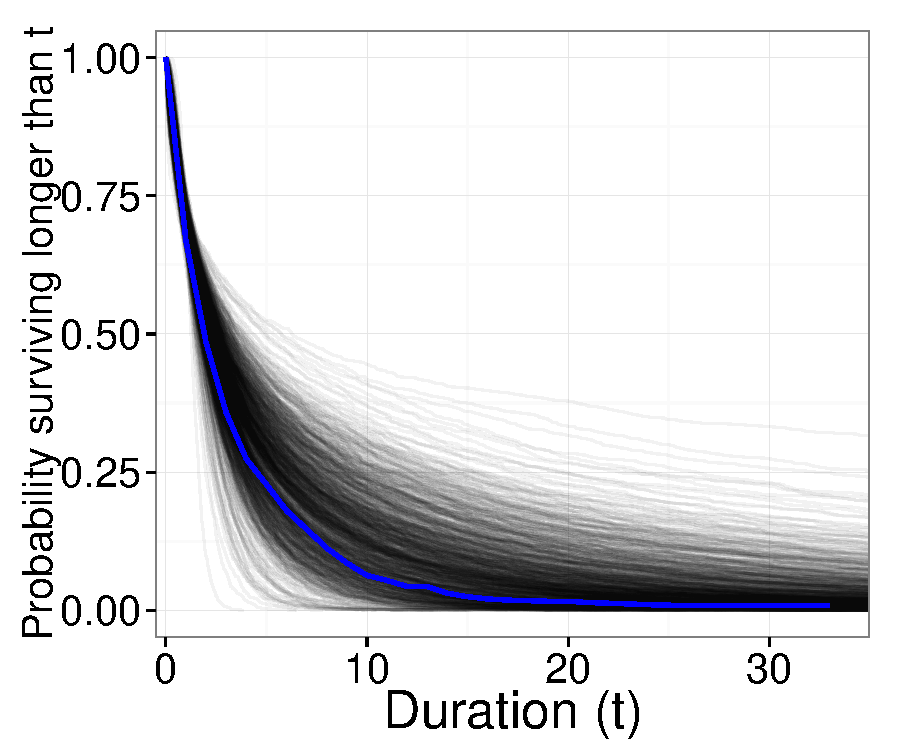
\includegraphics[height = 0.5\textheight,width=\textwidth,keepaspectratio=true]{figure/survival_curves}
  \caption{Comparison of empirical estimates of \(S(t)\) versus estimates from 1000 posterior predictive data sets. \(S(t)\) corresponds to \(P(T > t)\) as it is the probability that a given genus observed at age \(t\) will continue to live. This is equivalent to the probability that \(t\) is less than the genus' ultimate duration \(T\). Note that the Weibull (left) model has noticeably better fit to the data than the exponential (right).}
  \label{fig:surv}
\end{figure}

\begin{figure}[ht]
  \centering
  \includegraphics[height = 0.5\textheight,width=\textwidth,keepaspectratio=true]{figure/environ_quad}
  \caption{The overall expected relationship \(f(v_{i})\) between environmental affinity \(v_{i}\) and a multiplier of extinction risk (Eq. \ref{eq:env}). Each grey line corresponds to a single draw from the posterior predictive distribution, while the black corresponds to the median of the posterior predictive distribution. The overall shape of \(f(v_{i})\) is concave down with an optimum of close 0, which corresponds to affinity approximately equal to the expectation based on background environmental occurrence rates.}
  \label{fig:env_mean}
\end{figure}


\begin{figure}[ht]
  \centering
  \begin{subfigure}[b]{0.5\textwidth}
    \caption{}
    \includegraphics[height = 0.5\textheight,width=\textwidth,keepaspectratio=true]{figure/wei_cor_heatmap}
    \label{fig:omega}
  \end{subfigure}
  \begin{subfigure}[b]{0.4\textwidth}
    \caption{}
    \includegraphics[height = 0.5\textheight,width=\textwidth,keepaspectratio=true]{figure/correlation_marginal}
    \label{fig:corr}
  \end{subfigure}
  \caption{\textbf{A}: Heatmap for the median estimates of the terms of the correlation matrix \(\Omega\) between cohort-level covariate effects. Both the exponential (left) and Weibull (right) models are presented. The off-diagonal terms are the correlation between the estimates of the cohort-level estimates of the effects of covariates, along with intercept/baseline extinction risk. \textbf{B}: Marginal posterior distributions of the correlations between intercept terms/baseline extinction risk and the effects of each of the covariates. These are presented for both the exponential (left) and Weibull (right) models.}
  \label{fig:cor_posterior}
\end{figure}


\begin{figure}[ht]
  \centering
  \begin{subfigure}[b]{\textwidth}
    \caption{}
    \includegraphics[width = \textwidth,keepaspectratio=true]{figure/intercept_cohort}
    \label{fig:cohort_intercept}
  \end{subfigure}

  \begin{subfigure}[b]{\textwidth}
    \caption{}
    \includegraphics[width = \textwidth,keepaspectratio=true]{figure/range_cohort}
    \label{fig:cohort_range}
  \end{subfigure}
  \caption{Comparison of cohort-specific estimates of \(\beta_{0}\) presented along with the estimate for the overall baseline extinction risk. Points correspond to the median of the cohort-specific estimate, along with 80\% credible intervals. The horizontal line is the median estimate of the overall baseline extinction risk along with 80\% credible intervals. Results are presented for the exponential (top) and Weibull (bottom) models. Comparison of cohort-specific estimates of the effect of geographic range on extinction risk \(\beta_{r}\) presented along with the estimate for the overall effect of geographic range. Points correspond to the median of the cohort-specific estimate, along with 80\% credible intervals. The horizontal line is the median estimate of the overall baseline extinction risk along with 80\% credible intervals. Results are presented for the exponential (top) and Weibull (bottom) models.}
  \label{fig:cohort_info}
\end{figure}


\begin{sidewaysfigure}[ht]
  \centering
  \includegraphics[height = 0.5\textheight,width=\textwidth,keepaspectratio=true]{figure/cohort_quads}
  \caption{Comparison of the cohort-specific estimates of \(f(v_{i})\) (Eq. \ref{eq:env}) for the 33 analyzed origination cohorts. The stage of origination is labeled on the x-axis of each panel. The oldest stage is in the upper left, while the youngest is in the lower left. The number in each panel corresponds to the posterior probability that \(f(v_{i})\) is concave down. Those that are highlighed in red have less than 51\% posterior predictive probability that \(f(v_{i})\) is concave down.}
  \label{fig:env_cohort}
\end{sidewaysfigure}

\begin{table}
  \centering
  \begin{tabular}{ l r r }
    \hline
    parameter & mean & standard deviation \\ 
    \hline
    \(\mu_{i}\) & -1.51 & 0.15 \\ 
    \(\mu_{r}\) & -1.38 & 0.14 \\ 
    \(\mu_{e}\) & -0.08 & 0.18 \\ 
    \(\mu_{e2}\) & 0.25 & 0.43 \\ 
    \(\mu_{m}\) & -0.09 & 0.09 \\ 
    \(\tau_{i}\) & 0.63 & 0.11 \\ 
    \(\tau_{r}\) & 0.48 & 0.12 \\ 
    \(\tau_{e}\) & 1.07 & 0.23 \\ 
    \(\tau_{e^{2}}\) & 1.88 & 0.66 \\ 
    \(\tau_{m}\) & 0.32 & 0.13 \\ 
    \hline
  \end{tabular}
  \caption{Group-level estimates of the intercept terms the effects of biological traits on brachiopod generic survival from equations \ref{eq:exp_total} and \ref{eq:wei_total}, presented as means and standard deviations. \(\mu\) values are the location parameters of the effects, while \(\tau\) values are the scale terms describing the variation between cohorts. The subscripts correspond to the following: \(i\) intercept, \(r\) geographic range, \(e\) environmental affinity, \(e^{2}\) environmental affinity squared, \(m\) body size.}
  \label{tab:param}
\end{table}

\clearpage

\appendix
\documentclass[12pt,letterpaper]{article}

\usepackage{amsmath, amsthm}
\usepackage{microtype, parskip}
\usepackage[comma,numbers,sort&compress]{natbib}
\usepackage{lineno}
\usepackage{docmute}
\usepackage{caption, subcaption, multirow, morefloats, rotating}
\usepackage{wrapfig}

\frenchspacing

\renewcommand{\thefigure}{S\arabic{figure}}
\renewcommand{\thetable}{S\arabic{table}}
\renewcommand{\theequation}{S\arabic{equation}}

\setcounter{figure}{0}
\setcounter{table}{0}

\captionsetup[subfigure]{position = top, labelfont = bf, textfont = normalfont, singlelinecheck = off, justification = raggedright}

\title{Appendix for: The interplay between extinction intensity and selectivity: correlation in trait effects on taxonomic survival }

\begin{document}
\linenumbers
\modulolinenumbers[2]

\maketitle

\appendix
\section{Uncertainty in environmental preference} \label{sec:uncer}
The calculation and inclusion of environmental affinity in the survival model is a statistical procedure that takes into account our uncertainty based on where fossils tend to occur. Because we cannot directly observe if a fossil taxon had occurrences restricted to only a single environment, instead we can only estimate its affinity with uncertainty. One advantage of using a Bayesian analytical approach is that both parameters and data are considered random samples from some underlying distribution, which means that is is possible to model the uncertainty in our covariates of interest \citep{Gelman2013d}. My approach is conceptually similar to \citet{Simpson2009} but instead of obtaining a single point estimate, an entire posterior distribution is estimated.

The first step is to determine the probability \(\theta\) at which genus \(i\) occurs in an epicontinental setting based on its observed pattern of occurrences. Define \(e_{i}\) as the number of occurrences of genus \(i\) in an epicontiental sea and \(o_{i}\) as the number of occurrences of genus \(i\) not in an epicontinental sea (e.g. open ocean). Because the value of interest is the probability of occurring in an epicontinental environment, given the observed fossil record, I assume that probability follows a Bernoulli distribution. We can then define our sampling statement as
\begin{equation}
  e_{i} \sim \mathrm{Bernoulli}(e_{i} + o_{i}, \theta_{i}).
  \label{eq:epi_lik}
\end{equation}
I used a flat prior for \(\theta_{i}\) defined as \(\theta_{i} \sim \mathrm{Beta}(1, 1)\). Because the beta distribution is the conjugate prior for the Bernoulli distribution, the posterior is easy to compute in closed form. The posterior probability of \(\theta\) is then 
\begin{equation}
  \theta_{i} \sim \mathrm{Beta}(e_{i} + 1, o_{i} + 1)
  \label{eq:epi_post}
\end{equation}

It is extremely important, however, to take into account the overall environmental occurrence probability of all other genera present at the same time as genus \(i\). This is incorporated as an additional probability \(\Theta\). Define \(E_{i}\) as the total number of other fossil occurrences (exceptfor genus \(i\)) in epicontinental seas during stages where \(i\) occurs and \(O_{i}\) as the number of other fossil occurrences not in epicontinental seas. We can then define the sampling statement as
\begin{equation}
  E_{i} \sim \mathrm{Bernoulli}(E_{i} + O_{i}, \Theta_{i}).
  \label{eq:bck_lik}
\end{equation}
Again, I used a flat prior of \(\Theta_{i}\) defined as \(\Theta_{i} \sim \mathrm{Beta}(1, 1)\). The posterior of \(\Theta\) is then simply defined as

\begin{equation}
  \Theta_{i} \sim \mathrm{Beta}(E_{i} + 1, O_{i} + 1)
  \label{eq:bck_post}
\end{equation}

I then define the environmental affinity of genus \(i\) as \(v_{i} = \theta_{i} - \Theta_{i}\). \(v_{i}\) is a value that can range between -1 and 1, where negative values indicate that genus \(i\) tends to occur more frequently in open ocean environments than background while positive values indicate that genus \(i\) tends to occur in epicontiental environments.

While this approach is noticeably more complicated than previous ones \citep{Foote2006,Miller2001,Simpson2009,Kiessling2007a} there are some important benefits to both using a continuous measure of affinity as well directly modeling our uncertainty. In order to show some of these benefits, I performed a simulation analysis of modal/maximum \textit{a posteriori} (MAP) estimates versus full posterior estimates.

In this simulation, I first defined the ``background'' epicontinental occurrence \(\theta_{b}\) as 0.50 with a small amount of noise. This was represented as a beta distribution 

\begin{equation}
  \Theta_{b} = \mathrm{Beta}(\alpha = 2500, \beta = 2500). 
  \label{eq:bck_sim}
\end{equation}
This choice of parameters for the distribution reflects the average number of background occurrences for either epicontinental or open ocean environments per genus.

Using this background occurrence ratio, I randomly generated the occurrence patterns of 1000 simulated taxa. This was done at multiple sample sizes (1, 2, 3, 4, 5, 10, 25, 50, 100) in order to demonstrate the effects of increasing sample size on the confidence of environmental affinity. For each simulated taxon I calculated the full posterior distribution while assuming a flat Beta prior (\(\mathrm{Beta}(1, 1)\)). Using the full posterior I calculated the MAP probability of occurring in epicontinental environments. The environmental affinity was calculated for each of the simulated taxa using both the full posterior and the MAP estimate. In this toy example, environmental affinity can range between -0.5 and 0.5.

As should be expected, as sample size increases the distribution of MAP estimates converge on the true value (Fig. \ref{fig:env_mode}). For taxa with less than 10 occurrences, the MAP estimate is biased towards extreme values. Note that the mode of the beta distribution is not defined for situations where there were 0 draws of one of the environmental conditions. Instead, the vertical line is based entirely on the observed occurrences which are technically the modal estimates because they are the most frequently occurring/highest density.

In contrast, we can compare the true occurrence probability distribution versus the posterior estimate for a given sample (Fig. \ref{fig:env_post}). When sample sizes are low, posterior estimates are flat and represent a compromise between the likelihood and the flat prior (Eq. \ref{eq:epi_post}). Because of this, estimates from small sizes are less likely to be overly biased towards the extremes. This is further emphasized by inspection of the estimates of environmental affinity for the simulated taxa (Fig. \ref{fig:env_diff}). Posterior estimates from simulated taxa with small sample size have a much broader distribution that both allows for the extreme observation but still captures the ``true'' value (0). 


By defining environmental preference as the difference in full posterior estimates of occurrence probability, it is possible to include taxa with low sample sizes that are normally discarded \citep{Foote2006,Miller2001,Simpson2009,Kiessling2007a}. Additionally, 55+\% of observed Paleozoic brachiopod genera have less than 10 occurrences which is the range of sample sizes where MAP (or ML) estimates would be potentially most biased. This is preferable to finding the difference between the MAP estimates (blue line; Fig. \ref{fig:env_diff}).

% behavior of MAP estimates
%   as sample size increases, converge on true (10+)
% behavior of posterior
%   compromise between likelihood of data occurrences and (flat) prior
%   really important for small sample sizes
%   at 10+ makes no difference anymore
%   this is also kind obvious from the estimates of \(v\)
% how many taxa have less than 10 occurrences? \approx 55\%

\begin{figure}[ht]
  \centering
  \includegraphics[height = \textheight,width=\textwidth,keepaspectratio=true]{figure/env_mode_dist}
  \caption{Histograms of the distributions from the beta distribution defined in Eq. \ref{eq:bck_sim}. As to be expected, as sample size increases the draws better resemble the underlying true distribution. Sample size is indicated as the label of the x-axis, increasing in column major order.}
  \label{fig:env_mode}
\end{figure}

\begin{figure}[ht]
  \centering
  \includegraphics[height = \textheight,width=\textwidth,keepaspectratio=true]{figure/env_post_inspect}
  \caption{Comparisons of the underlying distribution (blue) to posterior estimates based on increasing sample size (gold). Each posterior estimate is represented for only a single realization of draws, each with sample size indicated as the x-axis label (increasing in column major order). Black vertical lines correspond to the MAP estimate of the simulated taxon's affinity. This stands in contrast to the posterior distribution of expected affinity in gold.}
  \label{fig:env_post}
\end{figure}

\begin{figure}[ht]
  \centering
  \includegraphics[height = \textheight,width=\textwidth,keepaspectratio=true]{figure/env_diff}
  \caption{Histograms of the difference in the underlying occurrence distribution and the posterior distribution estimates from the previous graph (Fig. \ref{fig:env_post}). The ``true'' value is included in all distributions of environmental affinities. Each affinity estimate is represented for only a single realization of draws, each with sample size indicated as the x-axis label (increasing in column major order). Blue vertical lines correspond to the difference in MAP estimates between the underlying distribution and the simulated taxon's draws. This stands in contrast to the distribution of the differences between the simulated taxon and background.}
  \label{fig:env_diff}
\end{figure}


\section{Survival model} \label{sec:survival}

The simplest model of genus duration includes no covariate or structural information. Define \(y_{i}\) as the duration in stages of genus \(i\), where \(i = 1, \dots, n\) and \(n\) is the number of observed genera. These two models are them simply defined as
\begin{equation}
  \begin{aligned}
    y_{i} &\sim \mathrm{Exponential}(\lambda) \\
    y_{i} &\sim \mathrm{Weibull}(\alpha, \sigma).
  \end{aligned}
  \label{eq:simple}
\end{equation}
\(\lambda, \alpha, \text{and} \sigma\) are all defined for all positive reals. Note that \(\lambda\) is a ``rate'' or inverse-scale while \(\sigma\) is a scale parameter, meaning that \(\frac{1}{\lambda} = \sigma\).

These simple models can then be expanded to include covariate information as predictors by reparameterizing \(\lambda\) or \(\sigma\) as a regression \citep{Klein2003}. Each of the covariates of interest is given its own regression coefficient (e.g. \(\beta_{r}\)) along with an intercept term \(\beta_{0}\). There are some additional complications to the parameterization of \(\sigma\) associated with the inclusion of \(\alpha\) as well as for interpretability \citep{Klein2003}. Both of these are then written as
\begin{equation}
  \begin{aligned}
    \lambda_{i} &= \exp(\beta_{0} + \beta_{r} r_{i} + \beta_{v} v_{i} + \beta_{v^{2}} v_{i}^{2} + \beta_{m} m_{i}) \\
    \sigma_{i} &= \exp\left(\frac{-(\beta_{0} + \beta_{r} r_{i} + \beta_{v} v_{i} + \beta_{v^{2}} v_{i}^{2} + \beta_{m} m_{i})}{\alpha}\right).
  \end{aligned}
  \label{eq:regression}
\end{equation}
The quadratic term for environmental affinity \(v\) is to allow for the possible nonlinear relationship between environmental affinity and extinction risk.

The models which incorporate both equations \ref{eq:simple} and \ref{eq:regression} can then be further expanded to allow all of the \(\beta\) coefficients, including \(\beta_{0}\), to vary with origination cohort while also modeling their covariance and correlation. This is called a varying-intercepts, varying-slopes model \citep{Gelman2007}. It is much easier to represent and explain how this is parameterized using matrix notation. First, define \(\mathbf{B}\) as \(k \times J\) matrix of the \(k\) coefficients including the intercept term (\(k = 5\)) for each of the \(J\) cohorts. Second, define \(\mathbf{X}\) as a \(n \times k\) matrix where each column is one of the covariates of interest. Importantly, \(\mathbf{X}\) includes a column of all 1s which correspond to the constant term \(\beta_{0}\). Third, define \(j[i]\) as the origination cohort of genus \(i\), where \(j = 1, \dots, J\) and \(J\) is the total number of observed cohorts. We then rewrite \(\lambda\) and \(\sigma\) of equation \ref{eq:regression} in matrix notation as
\begin{equation}
  \begin{aligned}
    \lambda_{i} &= \exp(\mathbf{X}_{i} B_{j[i]}) \\
    \sigma_{i} &= \exp\left(\frac{-(\mathbf{X}_{i} B_{j[i]})}{\alpha}\right). 
  \end{aligned}
  \label{eq:multivariate}
\end{equation}

Because \(B\) is a matrix, I use a multivariate normal prior with unknown vector of means \(\mu\) and covariance matrix \(\Sigma\). This is written as 
\begin{equation}
  B \sim \mathrm{MVN}(\vec{\mu}, \Sigma)
  \label{eq:beta_prior}
\end{equation}
where \(\vec{\mu}\) is length \(k\) vector representing the overall mean of the distributions of \(\beta\) coefficients. \(\Sigma\) is a \(k \times k\) covariance matrix of the \(\beta\) coefficients.

I also allowed estimates of the Weibull shape parameter \(\alpha\) to vary hierarchically by cohort. Cohort-specific estimates of \(\alpha\) were considered exponentially-transformed exchangable draws from a shared normal distribution with mean \(a\) and standard deviation \(\pi\), both of which were given semi-informative (hyper)priors centered at \(\alpha = 1\) (\(a \sim \mathcal{N}(0, 1)\), \(\pi \sim \mathrm{C^{+}}(1)\)).

What remains is assigning priors the elements of \(\vec{\mu}\) and the covariance matrix \(\Sigma\). All elements of \(\vec{\mu}\) except for \(\mu_{r}\) were given horseshoe priors \citep{Carvalho2010,Carvalho2009} while \(\mu_{r}\) was given an informative normal prior (\(\mu_{r} \sim \mathcal{N}(-1, 1)\)). Horseshoe priors are strong regularizing priors with effectively infinite density at 0 and heavy, Cauchy-like tails \citep{Carvalho2010,Carvalho2009} which allow weakly inferred effects to be strongly drawn towards 0 while truly strong effects can remain large. The horseshoe prior consists of a normal distribution with scale term that is the product between a global shrinkage parameter \(\nu\) and a local shrinkage parameter \(\psi\) unique to each of the parameters of interest. These parameters are themselves given half-Cauchy priors (Eq. 1 and 2).

The prior for \(\Sigma\) is a bit more complicated due to its multivariate nature. Following the \citet{stan-manual:2014}, I modeled the scale terms separate from the correlation structure of the coefficients. This is possible because of the relationship between a covariance and a correlation matrix, defined as 
\begin{equation}
  \Sigma_{B} = \text{Diag}(\vec{\tau}) \Omega \text{Diag}(\vec{\tau})
  \label{eq:covcor}
\end{equation}
where \(\vec{\tau}\) is a length \(k\) vector of variances and Diag(\(\tau\)) is a diagonal matrix.

I used a LKJ prior distribution for correlation matrix \(\Omega\) as recommended by \citet{stan-manual:2014}. The LKJ distribution is a single parameter multivariate distribution where values of the parameter \(\eta\) greater than 1 concentrate density at the unit correlation matrix, which corresponds to no correlation between the \(\beta\) coefficients. The scale parameters, \(\vec{\tau}\), are given weakly informative half-Cauchy (C\(^{+}\)) priors following \citet{Gelman2006a}.



\section{Censored observations} \label{sec:cen}
A key aspect of survival analysis is the inclusion of censored, or incompletely observed, data points \citep{Ibrahim2001,Klein2003}. The two classes of censored observations encountered in this study were right and left censored observations. Right censored genera are those that did not go extinct during the window of observation, or genera that are still extant. Left censored observations are those taxa for which we know only an upper limit on their duration.

In the context of this study, I considered all genera that had a duration of only one geologic stage to be left censored as we do not have a finer degree of resolution. 

The key function for modeling censored observations is the survival function, or \(S(t)\). \(S(t)\) corresponds to the probability that a genus having existed for \(t\) stages will not have gone extinct while \(h(t)\) corresponds to the instantaneous extinction rate at taxon age \(t\) \cite{Klein2003}. For an exponential model, \(S(t)\) is defined as
\begin{equation}
  S(t) = \exp(-\lambda t),
  \label{eq:exp_surv}
\end{equation}
and for the Weibull distribution \(S(t)\) is defined as
\begin{equation}
  S(t) = \exp\left(-\left(\frac{t}{\sigma}\right)^{\alpha}\right).
  \label{eq:wei_surv}
\end{equation}
\(S(t)\) is equivalent to the complementary cumulative distribution function, \(1 - F(t)\) \citep{Klein2003}. 

For right censored observations, instead of calculating the likelihood as normal (Eq. \ref{eq:multivariate}) the likelihood of an observation is evaluated using \(S(t)\). Conceptually, this approach calculates the likelihood of observing a taxon that existed for at least that long. For left censored data, instead the likelihood is calculated using \(1 - S(t)\) which corresponds to the likelihood of observing a taxon that existed no longer than \(t\).

The full likelihood statements incorporating fully observed, right censored, and left censored observations are then
\begin{equation}
  \begin{aligned}
    \mathcal{L} &\propto \prod_{i \in C} \mathrm{Exponential}(y_{i} | \lambda) \prod_{j \in R} S(y_{j} | \lambda) \prod_{k \in L} \left(1 - S(y_{k} | \lambda)\right) \\
    \mathcal{L} &\propto \prod_{i \in C} \mathrm{Weibull}(y_{i} | \alpha, \sigma) \prod_{j \in R} S(y_{j} | \alpha, \sigma) \prod_{k \in L} \left(1 - S(y_{k} | \alpha, \sigma)\right)
  \end{aligned}
  \label{eq:censored_likelihood}
\end{equation}
where \(C\) is the set of all fully observed taxa, \(R\) the set of all right censored taxa, and \(L\) the set of all left-censored taxa.


\section{Widely applicable information criterion} \label{sec:waic}
WAIC can be considered a fully Bayesian alternative to the Akaike information criterion, where WAIC acts as an approximation of leave-one-out cross-validation which acts as a measure of out-of-sample predictive accuracy \citep{Gelman2013d}. WAIC is calculated starting with the log pointwise posterior predictive density calculated as
\begin{equation}
  \mathrm{lppd} = \sum_{i = 1}^{n} \log \left(\frac{1}{S} \sum_{s = 1}^{S} p(y_{i}|\Theta^{S})\right),
  \label{eq:lppd}
\end{equation}
where \(n\) is sample size, \(S\) is the number posterior simulation draws, and \(\Theta\) represents all of the estimated parameters of the model. This is similar to calculating the likelihood of each observation given the entire posterior. A correction for the effective number of parameters is then added to lppd to adjust for overfitting. The effective number of parameters is calculated, following the recommendations of \citet{Gelman2013d}, as
\begin{equation}
  p_{\mathrm{WAIC}} = \sum_{i = 1}^{n} V_{s = 1}^{S} (\log p(y_{i}|\Theta^{S})).
  \label{eq:pwaic}
\end{equation}
where \(V\) is the sample posterior variance of the log predictive density for each data point.

Given both equations \ref{eq:lppd} and \ref{eq:pwaic}, WAIC is then calculated
\begin{equation}
  \mathrm{WAIC} = \mathrm{lppd} - p_{\mathrm{WAIC}}.
  \label{eq:waic}
\end{equation}
When comparing two or more models, lower WAIC values indicate better out-of-sample predictive accuracy. Importantly, WAIC is just one way of comparing models. When combined with posterior predictive checks it is possible to get a more complete understanding of a model's fit to the data.

\clearpage

\bibliographystyle{evolution}
\bibliography{newbib,packages}

\end{document}



\end{document}
